\openingarticle
\def\ppages{\pagerange{Garcia:firstpage}{Garcia:lastpage}}
\def\shorttitle{Social Space in the Upper Palaeolithic}
\def\maintitle{The Management of Social Space in the Upper Palaeolithic: Patterns, Statistics, and Open GIS in the Lower Gallery of La Garma  (Cantabria, Northern Iberian Peninsula)}
\def\shortauthor{Camilo Barcia García}
\def\authormail{camilobarciagarcia@gmail.com}
\def\thanknote{\footnote{Camilo Barcia García obtained his BA in History in 2012 at Autonomous University of Barcelona (UAB). In 2013, he obtained a MA in Prehistory and Archaeology, with specialization in intra-site spatial analysis, at the University of Cantabria. Back in UAB, he earned a MA in Teacher Formation for High School Education on Social Sciences. Since 2012, he has been working on several projects as a collaborator and independent researcher, with a focus on spatial and virtual archaeology.}}
\def\affiliation{Independent Scholar, Research from a Master at the University of Cantabria (2013)}
%--------------------------------------------------------------
\mychapter{\maintitle}
\begin{center}
	{\Large\scshape\shortauthor \thanknote}\\[1em]
	\email \\
	\affiliation
\end{center}
\vspace{3em}
\midarticle
%--------------------------------------------------------------
\label{Garcia:firstpage}
\sisetup{%
	range-phrase ={--},%
}
%----------------------------------------------------
\begin{myabstract}
	Applications\marginnote{Abstract\\(In Spanish see below)} of intra-site spatial statistics decreased during the 1990s and early 2000s, reducing spatial analysis to refitting and density maps, thus leaving apart many interesting quantitative approaches. During the past 10 years, intra-site studies have increased their relevance due to the capabilities of Geographic Information Systems (GIS) and computer visualization. This paper recovers a few old concepts, such randomness or classical statistics, and incorporates them to more recent advances, such GIS, Open-Source Software (OSS), explorative analysis and geostatistical thought. These methods are applied to a lithic assemblage from the Lower Gallery of La Garma (Upper Palaeolthic cave site in Cantabria, Spain), where contexts are well-preserved, aiming to infer about human spatial behaviour from lithic distribution. I argue that there is a certain degree of spatial rationality behind actions in this site, and I explore its relationship with further dimensions of human activity. Due to lithic distribution and its relationship to other evidences (structures), temporal variation in the use of social space is proposed as hypothesis.

	\keywords[Palabras claves]{Intra-site, Spatial statistics, Open-source software, QGIS, Upper Palaeolithic.}
\end{myabstract}
	
%\section{Introduction: precedents and insights about intra-site spatial analysis}
\lettrine[lines=3,slope=4pt,findent=-3pt]{A}{s} a concept,\marginnote{Precedents and insights about intra-site spatial analysis} spatial archaeology is coterminous with archaeology itself. Spatial dimension becomes an omnipresent environment for all human actions, and in archaeological research all sources of evidences must be located and integrated: stratigraphic relations, sites, landscapes, artefacts or others. The synergy between logical positivism, multidisciplinary, highly technical approaches, quantitative data analysis, and functional explicative theories led to the development of the \emph{New Archaeology} during the 1960s and 70s. This paradigm became the real turning point of what we know now as \emph{intra-site spatial analysis}, introducing important changes in the methods applied (spatial statistics) and the explanatory models for social behaviour (ethnographic data). 
	
The beginnings of analytical spatial archaeology can be traced back to the 1970s, when Robert \textcite{Whallon_1973} introduced the basic concept of randomness as a comparative tool to study spatial distributions of artefacts, and David L. \textcite{Clarke_1997} formalized the definition for spatial archaeology as the study of human groups through the spatial relationships between evidences. Due to an increased interest in the topic, many researchers developed several techniques in subsequent publications \parencites[e.g.][]{Hodder_1976}{Upham_1979}{Hietala_1984}{Blankholm_1991}. However, faced by certain limitations \parencite[cf.][]{Gamble_1991}, advances in quantitative spatial analysis were gradually disregarded in favour of simpler density maps and formative inferences, more often taphonomic than social. During the twenty-first century, major improvements have been developed as a result of the generalized use of GIS and digital tools, in addition to a raising application of geomatic technologies and the development of integrative frameworks \parencites{Llobera_2011}{McCoy_2009}. Therefore, geostatistical approaches and analytical visualizations are earning importance, mainly boosted by user-friendly software and interdisciplinary research \parencites[e.g.][]{Barceló_2008}{Craig_2006}{Lloyd_2004}{Katsianis_2008}. Nonetheless, instead of some common trends in this field \parencite[see][]{Djindjian_1999}, intra-site archaeology stays without a standardised methodology yet, leading a huge but enriching diversification of methods and perspectives. 
	
	This paper aims to: (1) recover the concept of randomness as an extremely valuable tool to explore spatial distributions, (2) claim that descriptive statistics are useful to control second-order tests, (3) show the capabilities of Open-Source Software (OSS) to integrate different analytical stages, and (4) demonstrate that absence of protocols to analyse archaeological spaces is not necessarily a methodological weakness, provided that we address our questions and issues contextually in each case study.

%\section{Archaeological record: lithic remains and undisturbed occupation floors}

%\subsection{A case study from Magdalenian period:}

The \marginnote{Archaeological record: lithic remains and undisturbed occupation floors\\{A case study from Magdalenian period}}Lower Gallery of La Garma is an Upper Palaeolithic cave site in Cantabria, situated at \SI{55}{\metre} above mean sea level (AMSL), in the core of a karstic system (La Garma hill), \SI{5}{\kilo\metre} away from the Cantabrian coastline and \SI{11}{\kilo\metre} from the capital city of Santander (Fig. \ref{fig:Garcia_Fig1}a). The cave is about \SI{300}{\metre} long and has an extension of \SI{800}{\metre\square}. It has been divided into nine study areas, and maintains a constant altitude through many stances and passages (Fig. \ref{fig:Garcia_Fig1}b). The main site feature is its ancient entrance collapse, happened at some moment during the Late Glacial Maximum. Due to this, a broad variety of Palaeolithic evidences remained in the cave floor surface without sedimentary processes, producing that could be called a close “living floor” concept: rock and mobile art, lithic and bone industries, faunal and vegetal remains, structures and more, all of them left in their depositional context (but not necessary of anthropogenic origin) (Fig. \ref{fig:Garcia_Fig1}d-e). Nowadays, the access goes through two upper caves interconnected by chasms and galleries (La Garma A, La Garma B and Intermediate Gallery). Access is highly controlled for scientists and restricted for the main public \parencites{Arias_2011}{Maximiano_2013}{Ontañón_2003}.

\begin{figure}
	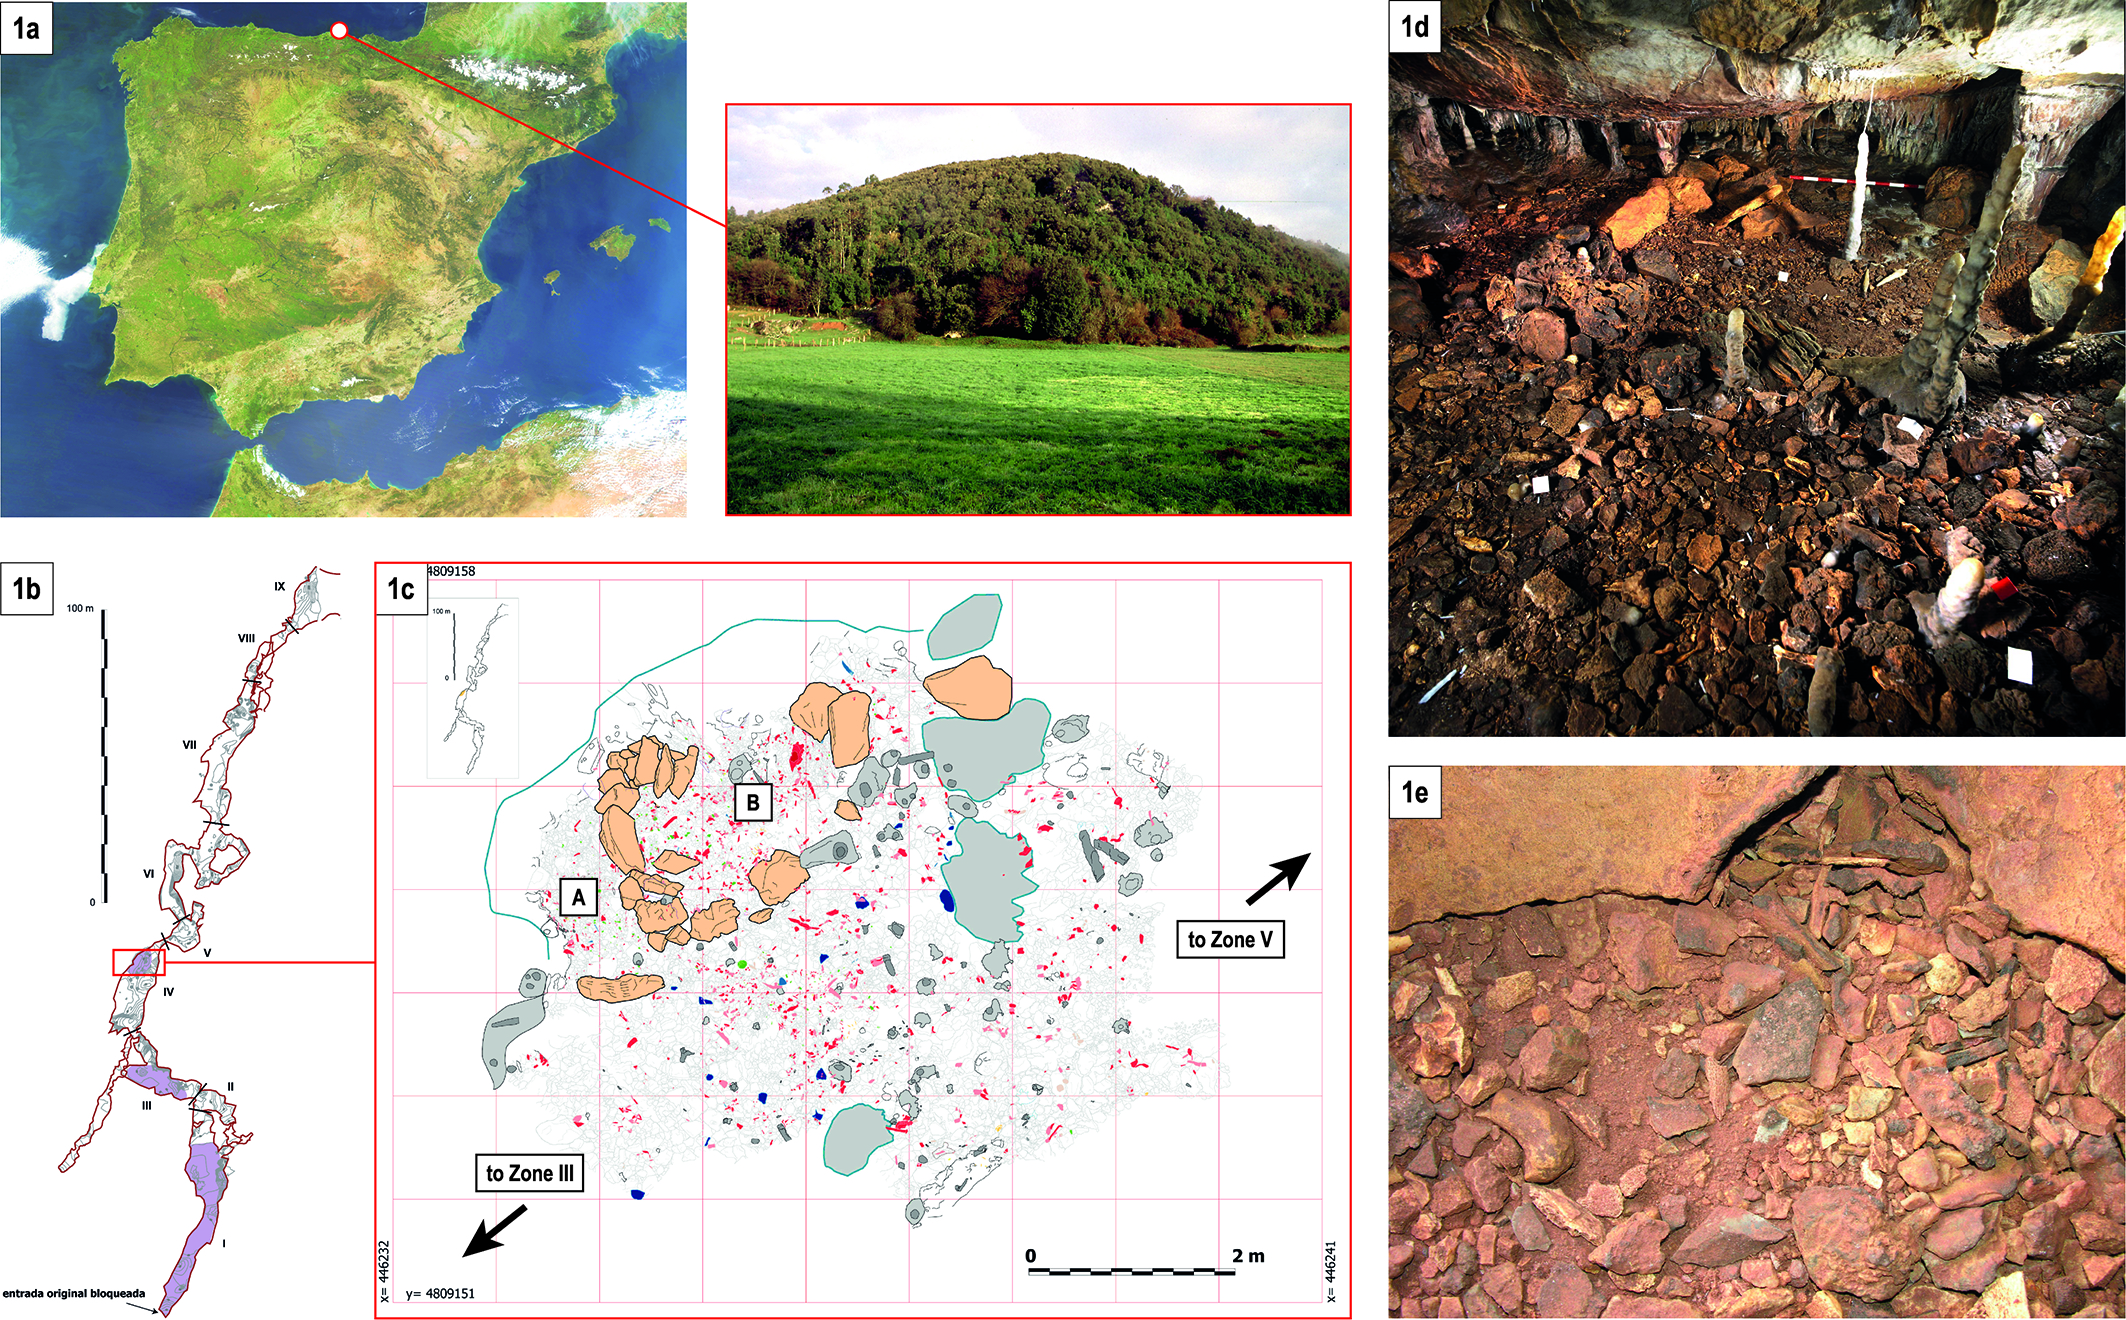
\includegraphics[width=\linewidth]{figures/garcia_Fig1}
	\caption{Geographical location of La Garma archaeological complex (1a); general map of Lower Gallery (1b); map of Zone IV (1c); general view of Zone IV (1d); detail of the occupation floor inside structure B (1e).}
	\label{fig:Garcia_Fig1}
\end{figure}

From a regional point of view, La Garma belongs to the Magdalenian culture (c.18-10kya) of the Upper Palaeolithic. This is a temporal context during which climate suffered a gradual but discontinue moderation, favouring the inhabitation of ecological niches on the littoral, river valleys and mountains, where human groups exploited some specific resources intensively (e.g. deer, chamois, river fishes, molluscs…) \parencites{Strauss_2010}{Utrilla_2004}. Flint and bone industries evolved from Solutrean to classic Cantabrian Magdalenian lithic and bone tools, the latter with animal decorations \parencites{González_2004}{Álvarez_2007}. A demographic increase seems well documented based on the intensity of cave occupations through time, and settlement patterning was oriented to the systematic catch of natural resources (i.e. minor specialized sites around base camps), partially related to “sanctuaries” with a broad presence of rock and mobile art, such as plaquettes, paintings, engravings, etc. \parencites{Strauss_1992}{Strauss_2010}. These cultural manifestations were also linked to a rich symbolic sphere and complex social relations \parencites{Arias_2009}{Schwendler_2012}. Long distance contacts to other peoples from the Pyrenees and south-western France have been suggested through the travelling of material, ideas, art, and probably also people \parencite{Sauvet_2008}.

This paper considers a particular area of the Lower Gallery of La Garma site: Zone IV. This sector is about \SI{130}{\meter} from the original entrance and the cave morphology maintains it away from sunlight. In Zone Iv, several rocks were disposed in a certain order forming closured spaces with low ceilings (no more than \SI{1.5}{\meter} high) and different floor composition (lower height and finer grained sediment), which have been defined as the structures A and B, extending over \SI{1.5}{\meter\squared} and \SI{3.18}{\meter\squared} respectively (see Fig. \ref{fig:Garcia_Fig1}c). Outside them, a larger space becomes a communicating passage between zones III and V (Fig. \ref{fig:Garcia_Fig1}b-c). Around \num{1200} lithics, \num{3750} bones and several kinds of vegetal remains (pollen, phytoliths…) are distributed over \SI{55}{\meter\squared}, inside and outside the structures (Fig. \ref{fig:Garcia_Fig1}d-e), associated to a chronology of 14300-14000 cal\BC \parencite{Arias_2011}. 
Research is still in progress. Thus, the following analysis aims to maximize inferences from the minor archaeological information available; in other words, this spatial analysis, with a reduced set of variables, could be helpful for further studies on prehistoric materiality and to more general spatial relationships within the site.

%\subsection{Hypotheses for lithic remains:}

Archaeological\marginnote{Hypotheses for lithic remains} evidences are the material expressions of human actions, motivated by social intentionality \parencite{Barceló_2002}, in accordance with cultural idiosyncrasies \parencite{Otte_2012}. The following analysis focuses on the lithic assemblage of Zone IV, in order to understand the social intentionality that distributes them through space, and how it relates to the human-made spatial limits represented by structures A and B \parencites{Kooyman_2006}{Maximiano_2008}. In order to construct an interpretative framework of social space from an archaeological context, we need to identify socio-spatially significant features on lithic distributions. If we consider site-formation processes \parencite[cf.][]{Schiffer_1976}, lithics passed from a systemic context to an archaeological one once they lose their functionality, regardless of whether their function was social, economic or symbolic. Lithics become socially excluded rubbish, discarded, abandoned and forgotten, and are then incorporated into the archaeological record \parencites{Clark_1991}{Hull_1987}{Murray_1980}{Schiffer_1976}. 

The lithic assemblage of Zone IV has been divided in two categories attending a basic contraposition: the spatial distribution of lithics that may have been useful after production and before abandonment (“Previous-Useful”: PU or artefacts), against the spatial distribution of objects that most likely were not useful after production (“Always-Useless”: AU or debris). During the knapping process, debris fall off from core and flakes, but due to their size, their passive role, and the stage of production in which are originated, they tend to be useless and left in place or moved away. After the knapping process, the flakes can be directly used, discarded, retouched or recycled, but by the end of their life-histories they’ll be equally discarded. The difference is that whereas “PU Objects” could be managed each one individually (one-by-one, just as artefacts), “AU Debris” tend to be managed collectively, by grouping or leaving apart many tiny remains at the same time. Since both categories can create dumping areas, they are different intentional contexts: lithic debris (AU) is directly related with knapping actions, so its location reveals activity areas or taphonomic events; while lithic objects (PU) are discarded as waste, and their spatial location could be related with (dumping) areas without any nuisance for culturally-accepted spatial ordering. Nonetheless, lithic disposals tend to follow social rules: dispersion indicates unconcern about refuse distribution in space, while accumulation implies cultural discrimination for dumping areas among the whole disposable space, relating that to those areas more frequently-usable or not for determinate activities. This can help to relate areas to particular activities or social behaviour.

The lithic assemblage of the Zone IV of Lower Gallery of La Garma has been divided into these two categories. The first one (objects PU) is composed by \num{316} remains bigger than \SIrange{7}{9}{\milli\meter}, including flakes, retouched tools, blades and bladelets, both broken and complete. The second category (debris AU) contains 853 tiny and shapeless fragments less than \SIrange{5}{7}{\milli\meter} in size, regardless whether their origin derives from knapping activities, taphonomic or other processes. These reflections and classification are inspired on very basic techno-morphological assumptions \parencites[see][]{Carbonell_1992}{Inizan_1999}{Mora_1992}, and entails just a preliminary and non-definitive approach to spatial identification of human actions and activity areas. 
Conclusions will be generalizations, and they may include some misleading or misclassified items, but the potential degree of error can be assumed without major impact on the interpretations. This way, we can obtain two possible conclusions at the level of social management of space: spatial segregation between activities can suggest further cultural rules in management of space; otherwise, superimposition of activities can suggest a socially polyvalent space (i.e. earlier actions not inhibit later ones).

%\section{GIS methods for ‘point patterns’}

As\marginnote{GIS methods for ‘point patterns’} previously stated, the introduction of randomness as analytical tool in spatial archaeology became a milestone, but it has arguably been underexploited. For the analysis of “point patterns” –i.e. spatial data given in the form of map coordinates–, randomness implies a non-significant variability in the values of a given variable according to its spatial location. In other words, the spatial location of a variable –e.g. a flake in a locus represented by three coordinates (XYZ)– may not have any relation with a major or minor presence of the same (or another) variable in its proximities, no matter how near or far could stay a second artefact from the first one. In fact, the sets of values in various locations are completely independent. Once a measure for randomness is obtained, variations and patterns in the spatial distribution can be spotted. So, if the occurrence probability increases the shorter the distance between artefacts is, and decreasing the larger de distance is –i.e. flakes are placed less distanced than what would be expected under random conditions–, it will be called “aggregate pattern”. On the contrary, if the occurrence probability for spatial distribution tends to decrease at short distances, and increasing at larger spatial separations, it will be called “disperse pattern”. These spatial dynamics are well-defined in mathematical terms, and are the basis to confirm or reject the Complete Spatial Randomness (CSR) hypothesis, being a helpful explorative approach that brings important information and enables further advanced analysis \parencites{Bailey_1995}{Bevan_2013}{Illian_2008}{Maximiano_2008}.

Several methods have been developed for the analysis of “point patterns”, many of them based on measures such as the inter-distance –i.e. separating distance between locations– or intensity –i.e. density, number of points by unit area–. One of the most popular is the Ripley’s K function, addressed to extract structural information including reduced second-order characteristics, that is, certain covariation at multiple scales. Nonetheless, centrographic statistical measures can be also applied as a first-order summary, in order to complete and control more specialized tests, such as Ripley’s K function. In addition, Kernel Density Estimators become a valuable graphical expression for intensity values.

\begin{labeling}{XXXXX}
\item[Centrographic Statistical Measures (CSM):] are composed by statistical measures, such as mean or standard deviation adapted, to two coordinates of “point patterns” (2D in a map). Mean becomes “centrographic mean” represented by a XY coordinate, while standard deviation becomes “standard distance” and is expressed as the radius of a circle which reflects degrees of dispersion \parencites{Ebdon_1985}{Wong_2005}. Although, the maximum extension of a distribution is indicated by the minimum polygon or “convex hull” that includes all points.
	
\item[Ripley’s K function (K-FUN):] cumulative function that compares intensity in an area of radius r against expected CSR values. A graphic output is displayed: if intensity is higher than random (aggregate trend) function shows a peak above the confidence interval, but if values are lower than random (disperse trend) function shows troughs under confidence interval \parencites{Orton_2004}{Wong_2005}. Confidence intervals are obtained from \num{999} Monte Carlo simulations, and results are exposed with and without edge effect corrections due to there is not any sample but a complete archaeological set. K-FUN needs to fix a study area, usually provided by the Minimum Enclosing Rectangle (MER) for the given “point pattern”: to facilitate further comparisons, study area for both categories will be the MER of the most extended distribution (“PU objects”) (see “Boundary layer” in Fig. \ref{fig:Garcia_Fig2}).

\item[Kernel Density Estimation (KDE):] probabilistic function that describes the intensity of points by displaying isolines according to a fixed radius and smoothing parameters \parencite{Baxter_1997}. KDE technique is a powerful visual complement to K-FUN (see \parencite[see][]{Sayer_2013}. In this case, parameters for KDE are \SI{20}{\centi\meter} radius and “quartic biweighted” for smoothing.

\item[Multivariate visualization:] analytic visualizations are valuable tools when we need to mix quantitative and qualitative spatial information; this way, the graphic plot of different variables or categories can be represented as trend surfaces, weighted quantities, or else \parencite{Craig_2006}. Hence, the procedure I have followed has been designed to express the spatial relevance of one category against other by unit area. Firstly, Zone IV is divided into a grid of equal quadrats (\SI{20}{\centi\meter} by side), and then each quadrat received a relative averaging measure. This last one is a percentage value calculated as follows; if the sum of “PU objects” and “AU debris” is \SI{100}{\percent} in every grid cell, the percentage of each category per quadrat can be obtained by cross-multiplication: that is, the multiplication of all the remains of just one category (PU or AU) by \num{100} and then divide it by the sum of all remains of both categories (e.g. if in a quadrat called x-1, there are “PU = 12” and “AU = 19”, then “PU + AU = 31”, thus “PU = [12*100] / 31 = \SI{38.71}{\percent}” and “AU = [19*100] / 31 = \SI{61.29}{\percent}”). As the whole grid needs to be calculated the same way, the estimation of just one category for all quadrats (PU or AU) will reflect the other one as its counterpart (e.g. if “PU = \SI{38.71}{\percent}”, then “AU = 100 – 38.71 = \SI{61.29}{\percent}”). Finally, grid is converted into regular point data by quadrat centroids and giving these centroids a corresponding percentage value; these values are interpolated by Inverse Distance Weighting (IDW) to obtain a trending surface. A \SIrange{45}{55}{\percent} average indicates non-meaningful relevancy of any specific category among other, but departures indicate areas where one category dominates among the other.  
\end{labeling}
%
\begin{figure}[!htb]
	\includegraphics[width=.7\linewidth]{figures/garcia_Fig2}
	\centering
	\caption{Overview of QGIS and its plugins (left). Ripley’s K function in R language (right).}
	\label{fig:Garcia_Fig2}
\end{figure}
GIS environments have a reputed efficiency for an integrated data management, analysis and visualization \parencites{Conolly_2006}{Wheatley_2002}. In this study, free OSS has been chosen, attending to both ethical and practical reasons: this kind of software neither charges user fees nor presents any restrictions in terms of licenses, it is a collective enterprise and it is usually user-friendly \parencite{Orengo_2015}. This way, QGIS provides all the analytic tools by itself, or through some plugins (e.g. PROCESSING) that connect the main program with other environments in order to increase its computing capacities (e.g. SAGA, GRASS, R, Python…). Thus, QGIS is used here for general management, CSM, KDE, and multivariate visualization; SAGA is used for CSM too; and R is used for K-FUN (Fig. \ref{fig:Garcia_Fig2}). R programming language also uses a specific package for spatial analysis called SPATSTAT, which permits to calculate the K function \parencites[see][]{Baddeley_2010}{Baddeley_2005}.


Supported on GIS environments, the analysis aims to seek paths to discover and analyze the variability of spatial distributions. The need to know how a distribution is and how it varies can be fulfilled by exploring its trends, patterns, variations between different observational scales, and other parameters. That must involve a well-suited relation among data nature, research aims and statistical techniques \parencites{Anselin_1999}{Bivand_2010}. At first, we use statistics and GIS to know how a spatial distribution of remains is. And then, infer what kind of human intention has generated that pattern. 

%\section{Results}

The\marginnote{Results} CSM for “AU debris” locates the centrographic mean on a flat stone in the SW of structure B, while significant part of them stays in a small area close to centrographic mean according to standard distance. Both centrographic mean and standard distance are displaced from the convex hull centre, giving the SW corner of structure B a significant role above the whole distribution. It seems clear that past social intentionality did not have the same degree of incidence in all possible locations of study area, but the gravity centre is conditioned by a high concentration on the flat stone. This fact will bias further analysis and must be considered: if we remove these \num{467} elements, centrographic mean is quite similar but standard distance circle grows, although most remains stays inside structures (Fig. \ref{fig:Garcia_Fig3}).

\begin{figure}
	\includegraphics[width=\linewidth]{figures/garcia_Fig3}
	\centering
	\caption{CSM plot for “AU debris”. Outlier corrections are in red.}
	\label{fig:Garcia_Fig3}
\end{figure}

KDE indicates that CSM coincides with high intensity values. Moreover, minor concentrations can be detected around bigger ones: at first, the semi-circle with empty inner space nearby to greater concentration in SW corner of structure B; then, similar incipient pattern arises in the structure A but is cut by structure limits (Fig. \ref{fig:Garcia_Fig4}, see top). The presence of “AU debris” in the outer area is merely residual. K-FUN describes a conventional aggregated pattern in two phases (Fig. \ref{fig:Garcia_Fig4}, see bottom): firstly, an aggregating trend arises from early stages to middle ones (L ups to 0.70 between \SIrange{0.00}{0.55}{\metre}) due to high average density of lithic debris at closer distances for the whole set; finally, a decreasing random trend appears from middle stages to the end (L descend to 0.60 between \SIrange{0.55}{1.00}{\metre}) due to the lack of same lithic remain density at longer distances than the shorter. Both trends have relation to the higher intensity of points located inside structures and to the lower intensity placed outside.

\begin{figure}
	\includegraphics[width=\linewidth]{figures/garcia_Fig4}
	\centering
	\caption{KDE plot for “AU debris” (top). Graphic display of K function (bottom); outliers previously explained (SW corner of structure B) are not computed.}
	\label{fig:Garcia_Fig4}
\end{figure}

Centrographic mean for “PU objects” is \SI{0.38}{\metre} far from the “AU debris” one, also in the SW corner of structure B, but significant part of these objects are distributed through a larger area according to standard distance. While centrographic mean is displaced from the convex hull centre, standard distance reaches larger extension of total distribution than it seems: there’re \num{4} objects in the SE that force the total extension (outliers), diminishing and hiding the real relevance of CSM (Fig. \ref{fig:Garcia_Fig5}). Thus, if these \num{4} elements are not computed, extension of convex hull decreases but it doesn’t entails a significant change in the size of standard distance circle.

\begin{figure}
	\includegraphics[width=\linewidth]{figures/garcia_Fig5}
	\centering
	\caption{CSM plot for “PU objects”. Outlier corrections are in red.}
	\label{fig:Garcia_Fig5}
\end{figure}

KDE indicates that CSM places all high intensity values inside structures A and B, but some other lower intensity values outside too. Intensity values are constantly low outside, while specific locations inside have higher intensities than surrounding areas. Furthermore, the shape of high values in structure B extends between SW flat stone and northern border (Fig. \ref{fig:Garcia_Fig6}, see top). K-FUN describes a stabilized aggregated (Fig. \ref{fig:Garcia_Fig6}, see bottom): at first, an aggregating trend arises from early stages to middle ones (L ups to 0.42 between \SIrange{0.00}{0.51}{\metre}) due to a high average density of lithic remains at short distances for the whole set. Finally, as the “AU debris” case, the crescent aggregating trend is stopped by non-increasing intensity at larger scales, but in the case of “PU objects” a more compensated scattering than “AU debris” over the entire Zone IV (both inside and outside the structures) avoid the apparition of a random or disperse pattern (L keeps 0.40 between \SIrange{0.51}{1.00}{\metre}). Both increasing and stabilized trends are related to shorter and larger scales respectively, so higher densities of lithic objects are linked to accumulations inside the structures while the stabilized trend is caused by more (non-strictly random) scattered objects over the whole area outside the structures (see KDE in Fig. \ref{fig:Garcia_Fig6}, top).

\begin{figure}
	\includegraphics[width=\linewidth]{figures/garcia_Fig6}
	\centering
	\caption{KDE plot for “PU objects” (top). Graphic display of K function (bottom); outliers previously explained (the four SE elements) are not computed.}
	\label{fig:Garcia_Fig6}
\end{figure}

A relevant aspect for KDE and F-FUN comparison between “AU debris” and “PU objects” is the larger aggregation index shown in debris (L = 0.70) than that seen in the objects case (L = 0.42). Mathematically, in the case of K-FUN, theoretically finite aggregated patterns will show a former ascending trend (aggregation) before decline (dispersion), and this happens because the accumulation of points (at higher or same intensities) stops at some moment the longer the distance computed, then starts to be more dispersed due to most points are located nearer to others than farer \parencite{Maximiano_2008}. Anyway, if the reduction in point presence (intensity) is more gradual and smoothed than a classic aggregated pattern model, the natural declining trend will happen at longer distances than in the case of a strong aggregated one. What can be observed in K-FUN for “PU objects” is the stabilization of aggregation index: it cannot arise nor decline as a result of lower intensities at large scales, but this decrease is not enough to cause a random or disperse pattern yet (at these scales of observation: \SIrange{0}{1}{\metre}). On the other hand, debris K-FUN trends fits well to conventional conceptions of an aggregated pattern. 

Plotting “PU objects” (green gradient, \SIrange{55}{100}{\percent} domination) against “AU debris” (purple gradient, \SIrange{55}{100}{\percent}), it can be seen that one single type dominates some areas (Fig. \ref{fig:Garcia_Fig7}). Besides, areas of equality can be distinguished too (\SIrange{45}{55}{\percent}). 
Differences in sample size could bias important information (i.e. “AU debris” can hide “PU objects”), so it is worth pointing out the most items of both categories have presence inside the structures. Thus, Zone IV is divided in two major trends: “AU debris” dominates inside structures (in a range from 60 to \SI{100}{\percent}, but sharing space with “PU objects”) while “PU objects” clearly dominate outside (around \SIrange{80}{100}{\percent} over the area except in very few debris locations). 
Other trends take the form of small spaces shared by both categories around the largest aggregations (\SIrange{40}{60}{\percent}), and there is also a very limited presence of “AU debris” outside the structures, 
and of “PU objects” surrounding inner debris. It can be concluded that there is a significant distinction between inside and outside areas, their linkage with one category for each one, and then, a deep variation that coincides with structure limits.
 
\begin{figure}
	\includegraphics[width=\linewidth]{figures/garcia_Fig7}
	\centering
	\caption{IDW plot for “AU debris” against “PU objects”.}
	\label{fig:Garcia_Fig7}
\end{figure}

%\section{Interpretation}
Lithic\marginnote{Interpretation} remains in the Lower Gallery of La Garma are not randomly distributed in space. There is a spatial dynamic which trends to aggregate debris in particular areas with a very specific distribution, while potential tools (“PU objects”) are also aggregated in some areas but more dispersed over others. It implies that spatial patterns are scale-dependant: gravity centres (traced by CSM) give more relevance to lithics inside the structures than those located outside, so the aggregating patterns of both categories are more conditioned by elements distributed within structures than their respective outer ones. Pattern variation shown at larger scales is more linked to distribution changes in external area than in the space closed by structures (see K-FUN explanation about “PU” and “AU” comparison stated above); this way, social intentionality tended to aggregate lithic elements inside, while in the outside area these intentional actions were more dispersedly distributed. Furthermore, there is a strong correlation between lithics and spatial segmentation (structures): the most meaningful changes in spatial variability of lithics coincide with structure limits. Hence, social intentionality –that rules on human actions and its material effects– makes distinction over all available space (the whole Zone IV), locating activities differentially and producing the observed spatial pattern.

From an interpretative angle, lithic debris located inside the structures can be related to knapping areas not only because of their classic definition or implications, but due to their spatial expression too (see KDE plot in Fig. \ref{fig:Garcia_Fig4}): non-overlapping and well-defined small aggregations of debris in structure B, with a reduction in concentration intensity from the centre to their periphery \parencites[e.g.][]{Kvamme_1997}{Nadel_2001}{Newcomer_1980}. Additionally, many debris remains are over the flat stone of SW corner in structure B. On the  other hand, spatial meaning of lithic “PU objects” is more ambiguous: they could were discarded next to knapping area as direct refuse after débitage or they might have been disposed there after some use. Attending a spatial pattern like the grown of aggregation only until specific scale, as shown in K-FUN and KDE (see Fig. \ref{fig:Garcia_Fig6}), past social actions disposed lithic objects discerning different kind of areas: there is not only a distinction between inner and outer space for dumping actions, but also between inner spaces. As an example, the great majority of lithic objects in structure B is located in the SW lateral while other parts of structure are nearly empty, meanwhile remains are more scattered in the outside area as a result of actions that no conceives preferential locations there. 
The entire available space in Zone IV does not play the same role in allowing social actions; these are differentially distributed in space.

In previous reviews of this site, temporal issues on occupational floors of Zone IV has been pointed out \parencite[see][]{Arias_2011}; this way, synchrony of remains confronts the absence of sedimentary processes –which is commonly related to short-occupation episodes (remains are visible during long time)–, to long age periods revealed by radiocarbon dating methods \parencite[35--39]{Arias_2011}. That introduces a palimpsest factor to the site, which can impact to spatial relations between elements, structures and to inner/outer areas stated above; however, intra-site spatial analysis and spatiotemporal interpretative framework can help to identify possible biases and to avoid this kind of low-resolution aspects. For example, non-statistical elements as the arranged floor and small inner space of structure A for knapping or other activities (\SI{1.5}{\metre\square}) could suggest not a functional one, but a remnant of an earlier occupation previous to structure B. This argument is strengthen by the diffuse southern limits of structure A, and by the presence of lithic remains between the bends of rocks which separate both structures (see Fig. \ref{fig:Garcia_Fig3} and \ref{fig:Garcia_Fig5}). When statistical geospatial data is put in context, both spatial patterns of debris and objects increases doubts on synchrony in favour of the palimpsest hypothesis: the shape of two lithic distributions looks similar to those located on SW part of structure B, but disrupted by structural limits (see KDE in Fig. \ref{fig:Garcia_Fig4} and \ref{fig:Garcia_Fig6}). All of this could indicate a superposition of buildings upon early lithic remains. 

%\section{Concluding remarks}

This\marginnote{Concluding remarks} analysis leads us to some interesting questions and hypotheses: (a) the minimum number of occupational stages of the site, and whether there was a temporal evolution of social space; (b) what indicators can be sought in the material record –i.e. lithics and else– to detect different kind of actions (e.g. trampling, use-wear traces, chemical residues, marks on flat stone in an “anvil” way…), and locating them to confirm or reject spatial segregation; and (c) if certain actions, such as flint knapping were carried out there (in full darkness, surrounded by rock art and other evidences), which would require a complex social interpretation and maybe the consideration of symbolic dimension.

Further research in the Lower Gallery of La Garma is still ongoing, so any interpretation should be considered as provisional, as a set of hypotheses to be tested. Future research should aim to undertake a full spatial analysis of all remains and environmental information in this site, together with a spatial comparison with similar archaeological contexts in the region \parencites[see][]{Arias_2005}{Arias_2009}. 

This paper focuses on basic quantitative approaches to quantify differences in spatial analysis. I argue that focusing on density maps do not allow to fully understand spatial interaction: is not the same random than disperse or aggregate, so implications for social inferences are substantially different. Therefore, density maps should be combined with other statistical and spatial techniques in order to approach questions regarding the social implications of an assemblage’s distribution. Considerable efforts are being directed to providing archaeology with robust spatial methodologies, mostly imported from other sciences. Intra-site spatial analysis is a powerful instrument to study archaeological spaces and their past social significance. However, explanatory models and the characterisation of socio-spatially relevant features in materiality, linking social intentionality with observable spatial patterns, needs to be revisited and expanded. A common criticism to \emph{New Archaeology} and \emph{Processualism} has been Eurocentric aprioristic assumptions, rigid deductive reasoning and limited interpretations (in terms of scientific laws). These general laws imply the mechanical correlation of an evidence to just one or two possible interpretations for all cultural contexts, underestimating the role of historical processes and social relations in their own idiosyncrasy \parencites{Hodder_2003}{Trigger_2006}. That methodological correlation was called “Middle-range theory” –similar to “Observational archaeological theory” in the terminology of Marxist Archaeology–, and despite their limitations, it can be a starting point for future research. Spatial models for intra-site studies of human behaviour are not broadly developed yet, but they could evolve from classic models through the application of methods such as experimental archaeology, ethnoarchaeology, computer simulations, geostatistics, digital 3D environments, GIS and more geospatial tools. Moreover, after taking care of the \emph{post-processual} warnings about the nature and the applicability of the evidence, spatial models should be conceived and played for further interpretation in a more indirect and “socially ambitious” way: becoming \emph{an analytical aid} to further interpretations –e.g. describing parameters as spatial segregation, minor statistical trends, attraction and repulsion between actions, correlations…–, \emph{more than an interpretation itself} –e.g. spatial models and quantitative techniques that aprioristically fit some classic activity areas on a given spatial distribution…–. This second one should be the last step in research, rather than the first.

\myseparator
%\section{Acknowledgements }
This\marginnote{Acknowledgements } paper revisits my Master Thesis, defended at the University of Cantabria in October 2013. It would not have been possible without the support of Dr. A. Maximiano Castillejo and Dr. P. Arias Cabal. 
The R script posted in Figure \ref{fig:Garcia_Fig2} has been possible by some modifications inspired in the algorithms of V. Olaya and Y. Ryabov for F, G and K functions on QGIS. Furthermore, I am grateful to the invaluable help of the GIS online community and forums (\href{http://gis.stackexchange.com}{http://gis.stackexchange.com}). Thanks also to the editorial team for their corrections and comments. Errors are only mine. Suggestions on QGIS and R are welcomed. 


\begin{myabstract}
\foreignlanguage{spanish}{La\marginnote{Abstract (Spanish)} estadística espacial intra-site sufrió un descenso durante la década de 1990 e inicios de los 2000, reduciendo el análisis espacial a remontajes y mapas de densidades, lo que dejó de lado diversos e interesantes enfoques cuantitativos. A lo largo de los últimos 10 años, los estudios intra-site han recobrado su relevancia gracias a la capacidad de los Sistemas de Información Geográfica (SIG) y la visualización informática. El presente artículo recupera viejos conceptos como la aleatoriedad o la estadística clásica, y los une a avances más recientes como los SIG, el software libre, los análisis exploratorios y el pensamiento geoestadístico. Estos métodos se han aplicado a un conjunto lítico procedente de la Galería Inferior de La Garma (yacimiento en cueva del Paleolítico Superior de Cantabria, España), donde los contextos están bien conservados, para inferir sobre el comportamiento espacial humano a partir de la distribución de restos líticos. Se concluye que existe cierto grado de racionalidad espacial tras las acciones sociales en este yacimiento, y se explora su relación con otras dimensiones de la actividad humana. A partir de la distribución lítica y su relación con otras evidencias (estructuras), se propone como hipótesis la variación temporal en el uso del espacio social.}

	
\keywords[Palabras claves]{Intra-site, Estadística espacial, Software libre, QGIS, Paleolítico Superior.}

\end{myabstract}

	
%-------------------------------------------------------------------------
%	REFERENCE LIST
\printbibliography[heading=subbibnumbered] 
\label{Garcia:lastpage}
\sisetup{%
	range-phrase ={$\times$},%
}
%------------------------------------------------------------------------------
\closingarticle